% Drawing 154/06-31 -- folder 154, batch 06, archive page 117 (PDF page 118).
% Transcription: deux dessins en couleur : un « couloir » rectangulaire (bords vert clair et vert foncé, tirets verts) traversé de droites rouges, un arc rouge le fermant en haut, avec deux flèches vers la légende « au choix » ; même dessin, variante
% Kind: corridor closed by a red arc, two variants. Method 2 (schematic redraw from the facsimile). Status: ok.
% Notes: Two drawings of a corridor. First: light green sides (the left one straight, crossed near its top by an oblique light green stroke; the right one bent, with two short strokes forking from it), their upper parts overdrawn in dark green; a dark bottom line; a red lens between the two sides, made of three red arcs from one side to the other (bowed up, nearly straight, bowed down); three red strokes from the lens down to the bottom, the first a thin spindle; inside, a dashed dark green loop (a sagging line under the lens, then down the left side, along the bottom and up the right side); two arrows from the words « au choix » to the right side of the loop. Second, lower on the page: light green sides, each with a curved fork at its top, dark green on the forks and in a small loop where the red arc meets each side; a dark green bottom line; one solid sagging red arc from side to side and, above it, a dashed red arc of which only the two ends are drawn; three red strokes down to the bottom, the middle one a thin spindle (in the first drawing it is the left one); the same dashed dark green loop; two arrows from the loop towards the words « au choix » (the heads are at the words, where in the first drawing they are at the loop). Overlaid on the 400 dpi colour crop on 2026-11-12 and redrawn: the second drawing is no longer a copy of the first, the lens has its three arcs, the dashed loop its shape, and the arrows of the second drawing their place (they ran up to the first drawing). The struck words to the right of the first drawing are not drawn. Redrawn 2026-11-12 (issue 128): to check again. Overlay check 2026-11-13 (issue 128, Claude claude-opus-5-5): redraw compiled with tectonic and laid over the 402 ppi colour scan; read again on a millimetre grid. First drawing: the three red arcs of the lens lowered by 1 to 2 mm onto the ink (they meet the sides at (10.6,-29.6) and (49.6,-30.6)), the two sides of the red spindle given their own tops and bottoms, the two red strokes moved to x = 31 and 39.4, the dashed loop lowered by 1 mm, the bottom line and the side ends set at y = -44.5, the arrow heads put where they are on the page, the oblique light green stroke straightened onto its ink. Second drawing: the red arc lowered by up to 0.7 mm, the red strokes moved to x = 21 and 40, the red spindle widened to its ink (28.7 to 34.6), the dashed loop and the bottom line lowered to the page, the right side ended at (47.6,-100.8), the arrow tails moved onto the loop. Now matches the facsimile; the struck words right of the first drawing are words, not drawing, and stay out.
% Coordinates: 1 unit = 1 mm = 1/100 of the crop width (bbox in page fractions: [0.15, 0.135, 0.345, 0.285]).
% Redrawn by Claude (claude-fable-5-2), issue #128, 2026-11-12; not checked by a human; not compiled (no TeX in the session).
% Corrected by Claude (claude-fable-5-2) 2026-11-12 (issue #128): overlaid on the 400 dpi colour facsimile and redrawn from it, the two drawings separately. Not compiled. Status: ok.
% Checked by Claude (claude-opus-5-5) 2026-11-13 (issue #128): overlay on the 402 ppi colour facsimile, corrected, compiled with tectonic. Not checked by a human. Status: ok.
% Rights: reproduces part of the work -- behind RENDER_TRANSCRIPTS, never published by itself.
\documentclass[tikz,border=3pt]{standalone}
\usepackage{amsmath,amssymb}
\usetikzlibrary{patterns,arrows.meta}
\tikzset{Lg/.style={green!60!black!70}, Dg/.style={green!45!black}, Rd/.style={red!85!black}, pencil/.style={black!45}, struck/.style={black!35}, mpt/.style={circle,draw,inner sep=1.3pt}, pt/.style={circle,fill,inner sep=0.9pt}, opt/.style={circle,draw,fill=white,inner sep=1.1pt}}
\colorlet{Or}{orange!90!black}\colorlet{Ye}{yellow!80!orange}\colorlet{Lg}{green!60!black!70}\colorlet{Dg}{green!45!black}\colorlet{Br}{brown!80!black}\colorlet{Rd}{red!85!black}\colorlet{Bl}{blue!70!black}\colorlet{Gy}{black!40}
\begin{document}
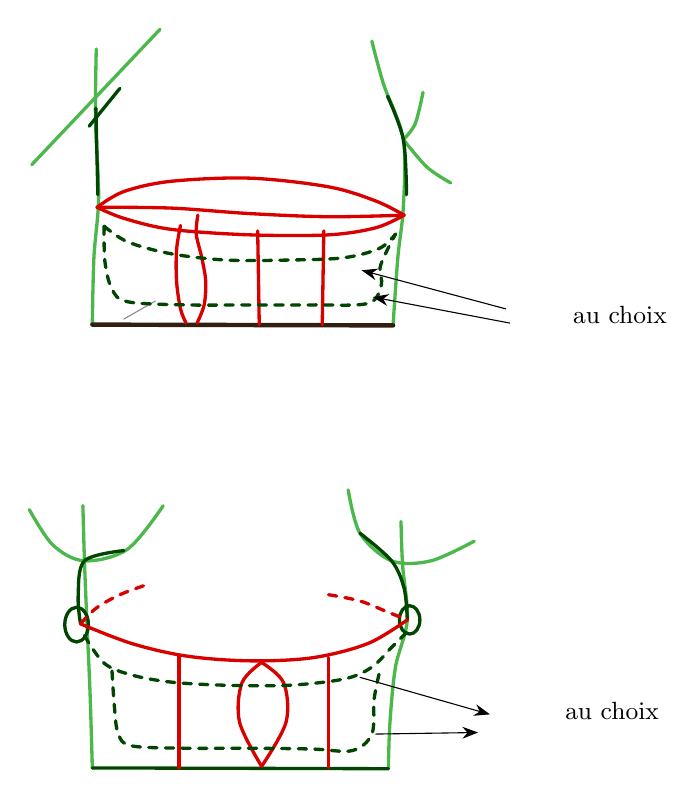
\begin{tikzpicture}[x=1mm,y=1mm,line cap=round,line join=round,font=\scriptsize]
\draw[Lg,very thick] plot[smooth, tension=0.55] coordinates {(10.5,-9.5) (10.4,-18.5) (10.8,-28.3) (10.2,-36) (10,-44.5)};
\draw[Lg,very thick] (2.3,-24.2) -- (18.6,-7);
\draw[Dg!60!black,very thick] (10.45,-17) -- (10.7,-28);
\draw[Dg!60!black,very thick] (9.6,-19.3) -- (13.5,-14.5);
\draw[Lg,very thick] plot[smooth, tension=0.55] coordinates {(45.5,-8.5) (47,-14) (49.5,-21) (49.5,-29.5) (48.8,-36) (48.2,-44.5)};
\draw[Lg,very thick] plot[smooth, tension=0.55] coordinates {(52,-15) (51,-19) (49.5,-21)};
\draw[Lg,very thick] plot[smooth, tension=0.55] coordinates {(49.5,-21) (52.5,-24.5) (55.5,-26.5)};
\draw[Dg!60!black,very thick] plot[smooth, tension=0.55] coordinates {(47.5,-15.5) (49.5,-21) (49.9,-28)};
\draw[black!75!brown,line width=1.6pt] (10,-44.5) -- (48.2,-44.6);
\draw[pencil] (14,-43.8) -- (18,-41.5);
\draw[Rd,very thick] plot[smooth, tension=0.55] coordinates {(10.6,-29.6) (14,-27.6) (20,-26.3) (30,-25.9) (40,-27) (46,-28.8) (49.6,-30.6)};
\draw[Rd,very thick] plot[smooth, tension=0.55] coordinates {(10.6,-29.6) (20,-29.7) (30,-30.4) (40,-30.8) (49.6,-30.6)};
\draw[Rd,very thick] plot[smooth, tension=0.55] coordinates {(10.6,-29.6) (14,-31) (20,-32.4) (30,-33.1) (40,-33.1) (46,-32.2) (49.6,-30.6)};
\draw[Rd,very thick] plot[smooth, tension=0.55] coordinates {(21.2,-31.9) (20.7,-35) (20.7,-39) (21.2,-42.5) (21.9,-44.3)};
\draw[Rd,very thick] plot[smooth, tension=0.55] coordinates {(23.4,-30.6) (23.2,-33) (23.9,-36) (24.4,-39) (24.2,-42) (23.3,-44.3)};
\draw[Rd,very thick] (31,-32.6) -- (31.2,-44.5);
\draw[Rd,very thick] (39.4,-32.6) -- (39.2,-44.5);
\draw[Dg!60!black,very thick,dashed] plot[smooth, tension=0.55] coordinates {(11.5,-32) (14.5,-34) (20,-35.5) (27,-36.3) (35,-36.3) (42,-36) (46.5,-34.8) (48.5,-33)};
\draw[Dg!60!black,very thick,dashed] plot[smooth, tension=0.55] coordinates {(11.5,-32) (11.6,-36.5) (12.5,-40) (14.5,-41.6) (22,-42) (30,-42) (38,-42) (45,-41.8) (46.7,-39.5) (46.6,-37) (48.5,-33)};
\draw[-{Stealth[length=2mm]}] (62.5,-42.5) -- (44.2,-37.6);
\draw[-{Stealth[length=2mm]}] (63,-44.3) -- (45.6,-41);
\node[inner sep=1pt] at (77,-43.3) {\small au choix};
\draw[Lg,very thick] plot[smooth, tension=0.55] coordinates {(8.8,-67.5) (9,-74.5) (9.3,-82) (9.7,-91) (10,-100.8)};
\draw[Lg,very thick] plot[smooth, tension=0.55] coordinates {(2,-68) (5,-72.5) (9,-74.5) (14.5,-73) (19,-67.5)};
\draw[Dg!60!black,very thick] plot[smooth, tension=0.55] coordinates {(14,-73.2) (9,-74.5) (8.2,-79) (8.5,-82.5)};
\draw[Dg!60!black,very thick] (8,-82.6) ellipse[x radius=1.5, y radius=2.2];
\draw[Lg,very thick] plot[smooth, tension=0.55] coordinates {(49.2,-69.5) (49.4,-75) (50,-82) (48.5,-88) (47.8,-95) (47.6,-100.8)};
\draw[Lg,very thick] plot[smooth, tension=0.55] coordinates {(42.5,-65.5) (44,-71) (48,-74.5) (53,-74.5) (58.5,-72)};
\draw[Dg!60!black,very thick] plot[smooth, tension=0.55] coordinates {(44,-71) (48,-74.5) (49.6,-78) (50,-82)};
\draw[Dg!60!black,very thick] (50.3,-82) ellipse[x radius=1.3, y radius=1.8];
\draw[Dg!60!black,very thick] (10,-100.8) -- (47.6,-100.9);
\draw[Rd,very thick] plot[smooth, tension=0.55] coordinates {(8.5,-82.5) (15,-85) (22,-86.6) (30,-87.2) (38,-86.8) (45,-85) (50,-82)};
\draw[Rd,very thick,dashed] plot[smooth, tension=0.55] coordinates {(8.5,-82.5) (10.5,-80.5) (13.5,-78.8) (17,-77.5)};
\draw[Rd,very thick,dashed] plot[smooth, tension=0.55] coordinates {(40,-78.8) (44,-79.6) (47.5,-81) (50,-82)};
\draw[Rd,very thick] (21,-86.5) -- (21,-100.8);
\draw[Rd,very thick] (40,-86.8) -- (40,-100.8);
\draw[Rd,very thick] plot[smooth, tension=0.55] coordinates {(31.5,-87.4) (29,-90) (28.7,-95) (31.5,-100.6)};
\draw[Rd,very thick] plot[smooth, tension=0.55] coordinates {(31.5,-87.4) (34.3,-90) (34.6,-95) (31.5,-100.6)};
\draw[Dg!60!black,very thick,dashed] plot[smooth, tension=0.55] coordinates {(9,-84) (11.5,-87.5) (15,-89) (20,-89.9) (27,-90.3) (35,-90.3) (42,-89.5) (45.5,-88) (48,-85.5) (50,-83.5)};
\draw[Dg!60!black,very thick,dashed] plot[smooth, tension=0.55] coordinates {(12.5,-88.5) (12.8,-93) (13.3,-96.5) (15,-98) (22,-98.3) (30,-98.3) (38,-98.4) (43,-98.6) (45.5,-96.5) (45.8,-92) (46.5,-88.5)};
\draw[-{Stealth[length=2mm]}] (44,-89.3) -- (60.5,-94);
\draw[-{Stealth[length=2mm]}] (46,-96.5) -- (59,-96.3);
\node[inner sep=1pt] at (76,-93.5) {\small au choix};
\end{tikzpicture}
\end{document}
